\documentclass[12pt,oneside]{book}

%%%%%%%%%%%%%%%%%%%%%%%%%%%%%%%%%%%%%%%%%%%%%%%%%%%%%%%%%%%%%%%%%%%%%%%%%%%%%%%%%%%%%%%%%%%%%%%%%%%
%                                                                                                 %
% The mathematical style of these documents follows                                               %
%                                                                                                 %
% A. Thompson and B.N. Taylor. The NIST Guide for the Use of the International System of Units.   %
%    NIST Special Publication 881, 2008.                                                          %
%                                                                                                 %
% http://www.nist.gov/pml/pubs/sp811/index.cfm                                                    %
%                                                                                                 %
%%%%%%%%%%%%%%%%%%%%%%%%%%%%%%%%%%%%%%%%%%%%%%%%%%%%%%%%%%%%%%%%%%%%%%%%%%%%%%%%%%%%%%%%%%%%%%%%%%%

\input{../../../../Bibliography/commoncommands}

% Load packages
\usepackage{graphicx}
\usepackage[super]{nth}
\usepackage{placeins}

% Rename chapter headings
\renewcommand{\chaptername}{Section}
\renewcommand{\bibname}{References}

% Math shortcuts
\renewcommand{\sb}[1]{_\mathrm{#1}}
\renewcommand{\C}{\mbox{C}}
\renewcommand{\H}{\mbox{H}}
\renewcommand{\O}{\mbox{O}}
\newcommand{\N}{\mbox{N}}

% Center all figures
\makeatletter
\g@addto@macro\@floatboxreset\centering
\makeatother

\begin{document}

\bibliographystyle{unsrt}
\pagestyle{empty}

\begin{minipage}[t][9in][s]{6.25in}

\headerB{
Impact of Hose Streams on Air Flows inside a Structure
}

\headerC{
\flushright{
Daniel Madrzykowski \\
Craig G. Weinschenk \\
Kristopher J. Overholt \\
{\em Fire Research Division \\
Engineering Laboratory \\
Gaithersburg, Maryland, USA} \\ }
}

\flushright{\today \\
}

\vfill

\flushright{
\includegraphics[width=2.in]{../../../../Bibliography/nistident_flright_vec} \\[.3in]
}

\titlesigs

\end{minipage}

\newpage

\frontmatter

\pagestyle{plain}
\pagenumbering{roman}

\cleardoublepage
\phantomsection
\addcontentsline{toc}{chapter}{Contents}
\tableofcontents

\cleardoublepage
\phantomsection
\addcontentsline{toc}{chapter}{List of Figures}
\listoffigures

\cleardoublepage
\phantomsection
\addcontentsline{toc}{chapter}{List of Tables}
\listoftables

\chapter{List of Acronyms}

\begin{tabbing}
\hspace{1.5in} \= \\
FDS \> Fire Dynamics Simulator \\
HGL \> Hot Gas Layer \\
HRR \> Heat Release Rate \\
HRRPUA \> Heat Release Rate per Unit Area \\
NIST \> National Institute of Standards and Technology \\
\end{tabbing}

\mainmatter

\chapter{Introduction}
\label{chap:Introduction}
NIST has conducted a significant amount of research examining how ventilation affects the growth and spread of fire within structures and how the air flow to the fire may be controlled to limit or delay the growth of the fire. The studies have resulted in guidance to the fire service regarding ventilation tactics. However, ventilation tactics alone will not result in the complete extinguishment of the fire; fire suppression with hose streams are needed.

Fire suppression tactics using hose streams also affect the ventilation in a structure and can impact the movement of smoke and heat through a structure as vents are made to advance the line or if ventilation inducing hand line tactics are in practice. This research addressing the coordination of suppression tactics and the impact on ventilation is needed to complete recommendations on fire control tactics to appropriate standards, education, and training documents.

This report is concerned with examining the impact of hose stream selection and the pattern in which the stream is applied on the ventilation inside a structure with various flow path configurations. Two types of experiments were conducted in order to examine the impact. First, cold flow tests were performed. These tests involved using a 0.46 m (18 in) diameter positive pressure ventilation (PPV) fan to move air through a structure with various flow path configurations. The second type of experiment involved flowing water using various stream and application patterns into a structure with flow path configurations similar to the cold flow test configurations. Air velocities measured during the hose flow experiments were compared to the velocities measured during the cold flow tests to determine the impact of hose stream and application pattern combinations on ventilation throughout the structure relative to the impact of using a 0.46 m (18 in) diameter PPV fan to move air throughout the structure. 

Three types of hose streams were each applied in four different fashions during each set of hose flow experiments. The three types of hose stream patterns studied, pictured in Figure~\ref{fig:hose_streams}, were straight stream, narrow fog stream, and wide fog stream. Water was flowed into the structure by having the hose in a static, fixed position, moving the hose line left-to-right across the room in a sweeping motion, and rotating the hose line in both the clockwise and counterclockwise directions.

\begin{figure}[!ht]
\includegraphics[width=6in]{../../Figures/hose_streams.pdf}
\caption[Different Hose Stream Patterns]{The three types of hose stream patterns, straight stream (left), narrow fog stream (middle), and wide fog stream (right), used during the water flow experiments.}
\label{fig:hose_streams}
\end{figure}
\FloatBarrier

\section{Background}
\label{sec:Background}


\chapter{Experimental Setup}
\label{chap:Experimental_Setup}

\section{Experimental Structure}
\label{sec:Experimental_Structure}
This series of field experiments was conducted into two structures located at the Delaware County Emergency Services Training Center in Sharon Hill, PA. 

\subsection{Construction}
\label{sec:Construction}
Two concrete structures were built on a concrete slab as shown in Fig.~\ref{fig:struct_pics}. They were designed to simulate a single story and a two story residential structure.  The first floor of each structure had an outer wall composed of interlocking concrete blocks 0.61 m (2 ft) wide, 0.61 m (2 ft) high and 1.22 m (4 ft) long. The interior dimensions of each structure were 6.1 m (20 ft) wide, 11 m (36 ft) long and 2.4 m (8 ft) high.  The joints and gaps between the blocks were filled with high temperature insulation.

The interior walls of the first floor or each structure were framed with steel studs and track.  The studs were set to 0.40 m (16 in) centers.  The ceiling/floor support was composed of wood truss joist I-beams (TJIs) with a 299 mm (11.75 in) depth.  The TJI was composed of laminated veneer lumber flanges with a cross section of 29 mm (1.125 in) x 44 mm (1.75 in) and an 11 mm (0.43 in) thick oriented strand board web as shown in Figure  XX .  Tongue and grove, 18.3 mm (0.72 in) thick, oriented strand board was screwed (nailed?) to the top of the TJIs.

The second story of the two level structure was built on the wood floor assembly as described above. The walls were framed with wood studs etc...

Opening front door, window, rear doors.  

Single story  
The interior walls of the burn room were lined with 13 mm (0.5 in) thick cement board.  The ceiling of the burn room was the exposed ``floor assembly".  The walls of the hallway and entry foyer were composed of 16 mm (0.625 in) Type X gypsum room. The ceiling of the hallway and entry foyer was composed of two layers of 13 mm (0.5 in) thick cement board.  

\begin{figure}[!ht]
\includegraphics[width=6in]{../../Figures/east_structure}
\\~\\
\includegraphics[width=6in]{../../Figures/west_structure}
\caption[East and West Test Structures]{East (top) and West (bottom) Test Structures}
\label{fig:struct_pics}
\end{figure}

\clearpage

\begin{figure}[!ht]
\includegraphics[trim=0cm 0cm 0.75cm 4.5cm, clip=true, width=6in]{../../Drawings/PDFs/Without_Instrumentation/West_Structure_1st_Floor_Metric_Simple}
\\
\includegraphics[trim=0cm 0cm 0.75cm 5.0cm, clip=true, width=6in]{../../Drawings/PDFs/Without_Instrumentation/West_Structure_2nd_Floor_Metric_Simple}
\caption[West Structure first and second floor layouts]{West Structure first floor (top) and second floor (bottom) layouts. All dimensions are in meters.}
\label{fig:west_general_plan}
\end{figure}

\clearpage

\section{Instrumentation}
\label{sec:Instrumentation}
Schematic plan overviews of the instrumentation in the East and West Structures are shown in Fig.~\ref{fig:east_instrumentation} and Fig.~\ref{fig:west_instrumentation}, respectively. There is a discussion of uncertainties for each measurement below in Section~\ref{sec:Uncertainty}. Gas velocity was measured at various doorways using differential pressure transducers connected to bi-directional velocity probes~\cite{McCaffrey:Combustion_and_Flame}. Each set of BDPs contained 8 probes located at distances of 0.08 m, 0.34 m, 0.61 m, 0.88 m, 1.15 m, 1.42 m, 1.68 m, and 1.95 m below the soffit of the corresponding doorway. Fig.~\ref{fig:BDPs} shows a picture of two sets of BDPs, A5 and A6, located at each double door on the first floor of the West Structure. A single thermocouple was attached to each bi-directional probe. The thermocouples used with the bi-directional probes are exposed-bead, Chromel-Alumel (type K) with a 1.0 mm (0.04 in) diameter. Starting with the exposed bead, the thermocouple wire was sheathed in a 3.2 mm (0.13 in) diameter Inconel shield, 0.76 m (2.5 ft) in length.

%\begin{figure}[!ht]
%\includegraphics[trim=0cm 0cm 0.75cm 4.5cm, clip=true, width=6in]{../../Drawings/PDFs/With_Instrumentation/East_Test_Structure_Devices_Hose_Test}
%\caption[Location of Instrumentation in East Structure]{Location of Instrumentation in East Structure}
%\label{fig:east_instrumentation}
%\end{figure}

\begin{figure}[!ht]
\includegraphics[trim=0cm 0cm 0.75cm 4.5cm, clip=true, width=6in]{../../Drawings/PDFs/With_Instrumentation/West_Test_Structure_Devices_Hose_Test_1st_Floor}
\\
\includegraphics[trim=0cm 0cm 0.75cm 5.0cm, clip=true, width=6in]{../../Drawings/PDFs/With_Instrumentation/West_Test_Structure_Devices_Hose_Test_2nd_Floor}
\caption[Location of Instrumentation in West Structure]{Location of Instrumentation in West Structure}
\label{fig:west_instrumentation}
\end{figure}

\begin{figure}[!ht]
\includegraphics[width=6in]{../../Figures/BDPs}
\caption[Two sets of BDPs in Doorway]{Two sets of BDPs, A5 and A6, in each doorway of the double doors on the first floor of the West Structure}
\label{fig:BDPs}
\end{figure}

\section{Uncertainty}
\label{sec:Uncertainty}
There are different components of uncertainty in the length, differential pressure, and gas velocity reported here. Uncertainties are grouped into two categories according to the method used to estimate them. Type A uncertainties are those which are evaluated by statistical methods, and Type B are those which are evaluated by other means ~\cite{Taylor&Kuyatt:1994}. Type B analysis of systematic uncertainties involves estimating the upper (+a) and lower (-a) limits for the quantity in question such that the probability that the value would be in the interval ($\pm$a) is essentially 100\%. After estimating uncertainties by either Type A or B analysis, the uncertainties are combined in quadrature to yield the combined standard uncertainty. Then, the combined standard uncertainty is multiplied by a coverage factor of two, which results in the expanded uncertainty with a 95\% confidence interval (2$\sigma$). For some of these components, such as the zero and calibration elements, uncertainties are derived from referenced instrument specifications. For other components, referenced research results and past experience with the instruments provided input in the uncertainty determination. 

Each length measurement was taken carefully. Length measurements such as the room dimensions,
instrumentation array locations, and fire apparatus (for example nozzle, sprinkler, or fan) placement were made with a hand held laser measurement device which is has an accuracy of $\pm6.0$ mm (0.24 in) over a range of 0.61 m (2.00 ft) to 15.3 m (50.0 ft)~\cite{Stanley}. However, conditions affecting the measurement, such as levelness of the device, yield an estimated uncertainty of $\pm$0.5\% for measurements in the 2.0 m (6.6 ft) to 10.0 m (32.8 ft) range. Steel measuring tapes with a resolution of $\pm$0.5 mm were used to locate individual sensors within a measurement array and to measure and position the furniture. The steel measuring tapes were manufactured in compliance with NIST Manual 44, which specifies a tolerance of $\pm1.6$ mm (0.06 in) for 9.1 m (30 ft) tapes and $\pm6.4$ mm (0.25 in) for 30.5 m (100 ft) tapes \cite{NIST_Manual_44}. Some issues, such as "soft" edges on the upholstered furniture, result in an estimated total expanded uncertainty of $\pm$1.0\%. 

Bi-directional probes and single thermocouples were used to measure the velocity. The bi-directional probes used similar pressure transducers as those used for the differential pressure measurements discussed above. Bare-bead Type K thermocouple are co-located with the probe. A gas velocity measurement study, examining the doorway flow of pre-flashover compartment fires, yielded expanded uncertainty measurements ranging from $\pm0.14$ to $\pm0.22$ for bi-directional probes of similar design \cite{Bryant:FSJ2009}. The total expanded uncertainty for gas velocity in these experiments estimated to be $\pm18$\%.   

Water flowrate was measured with a pressure and flow meter combination shown in Fig. \ref{fig:flow_meter}. The meter consists of a section of 6.35 cm (2.5 inch) cast aluminum pipe with a 0-4.1 MPa (0-600 psi) pressure transducer and a paddlewheel type flow sensor with a range of 0 to 4800 lpm (1250 gpm). The pressure transducer and paddlewheel both connect to the battery operated control box where the pressure transducer voltage is converted to a pressure and the paddlewheel pulse count is converted to a volumetric flow rate. The manufacturer reports a $\pm5$\% calibration expanded uncertainty for the flow sensor and $\pm3$\%  for the pressure sensor \cite{Akron}. The pressure transducer was calibrated with a known analog pressure gauge. The flow meter was calibrated by capturing water over time and measuring that mass of water to determine the flowrate. The total expanded uncertainty was estimated at $\pm10$\%. 

%\begin{figure}[!ht]
%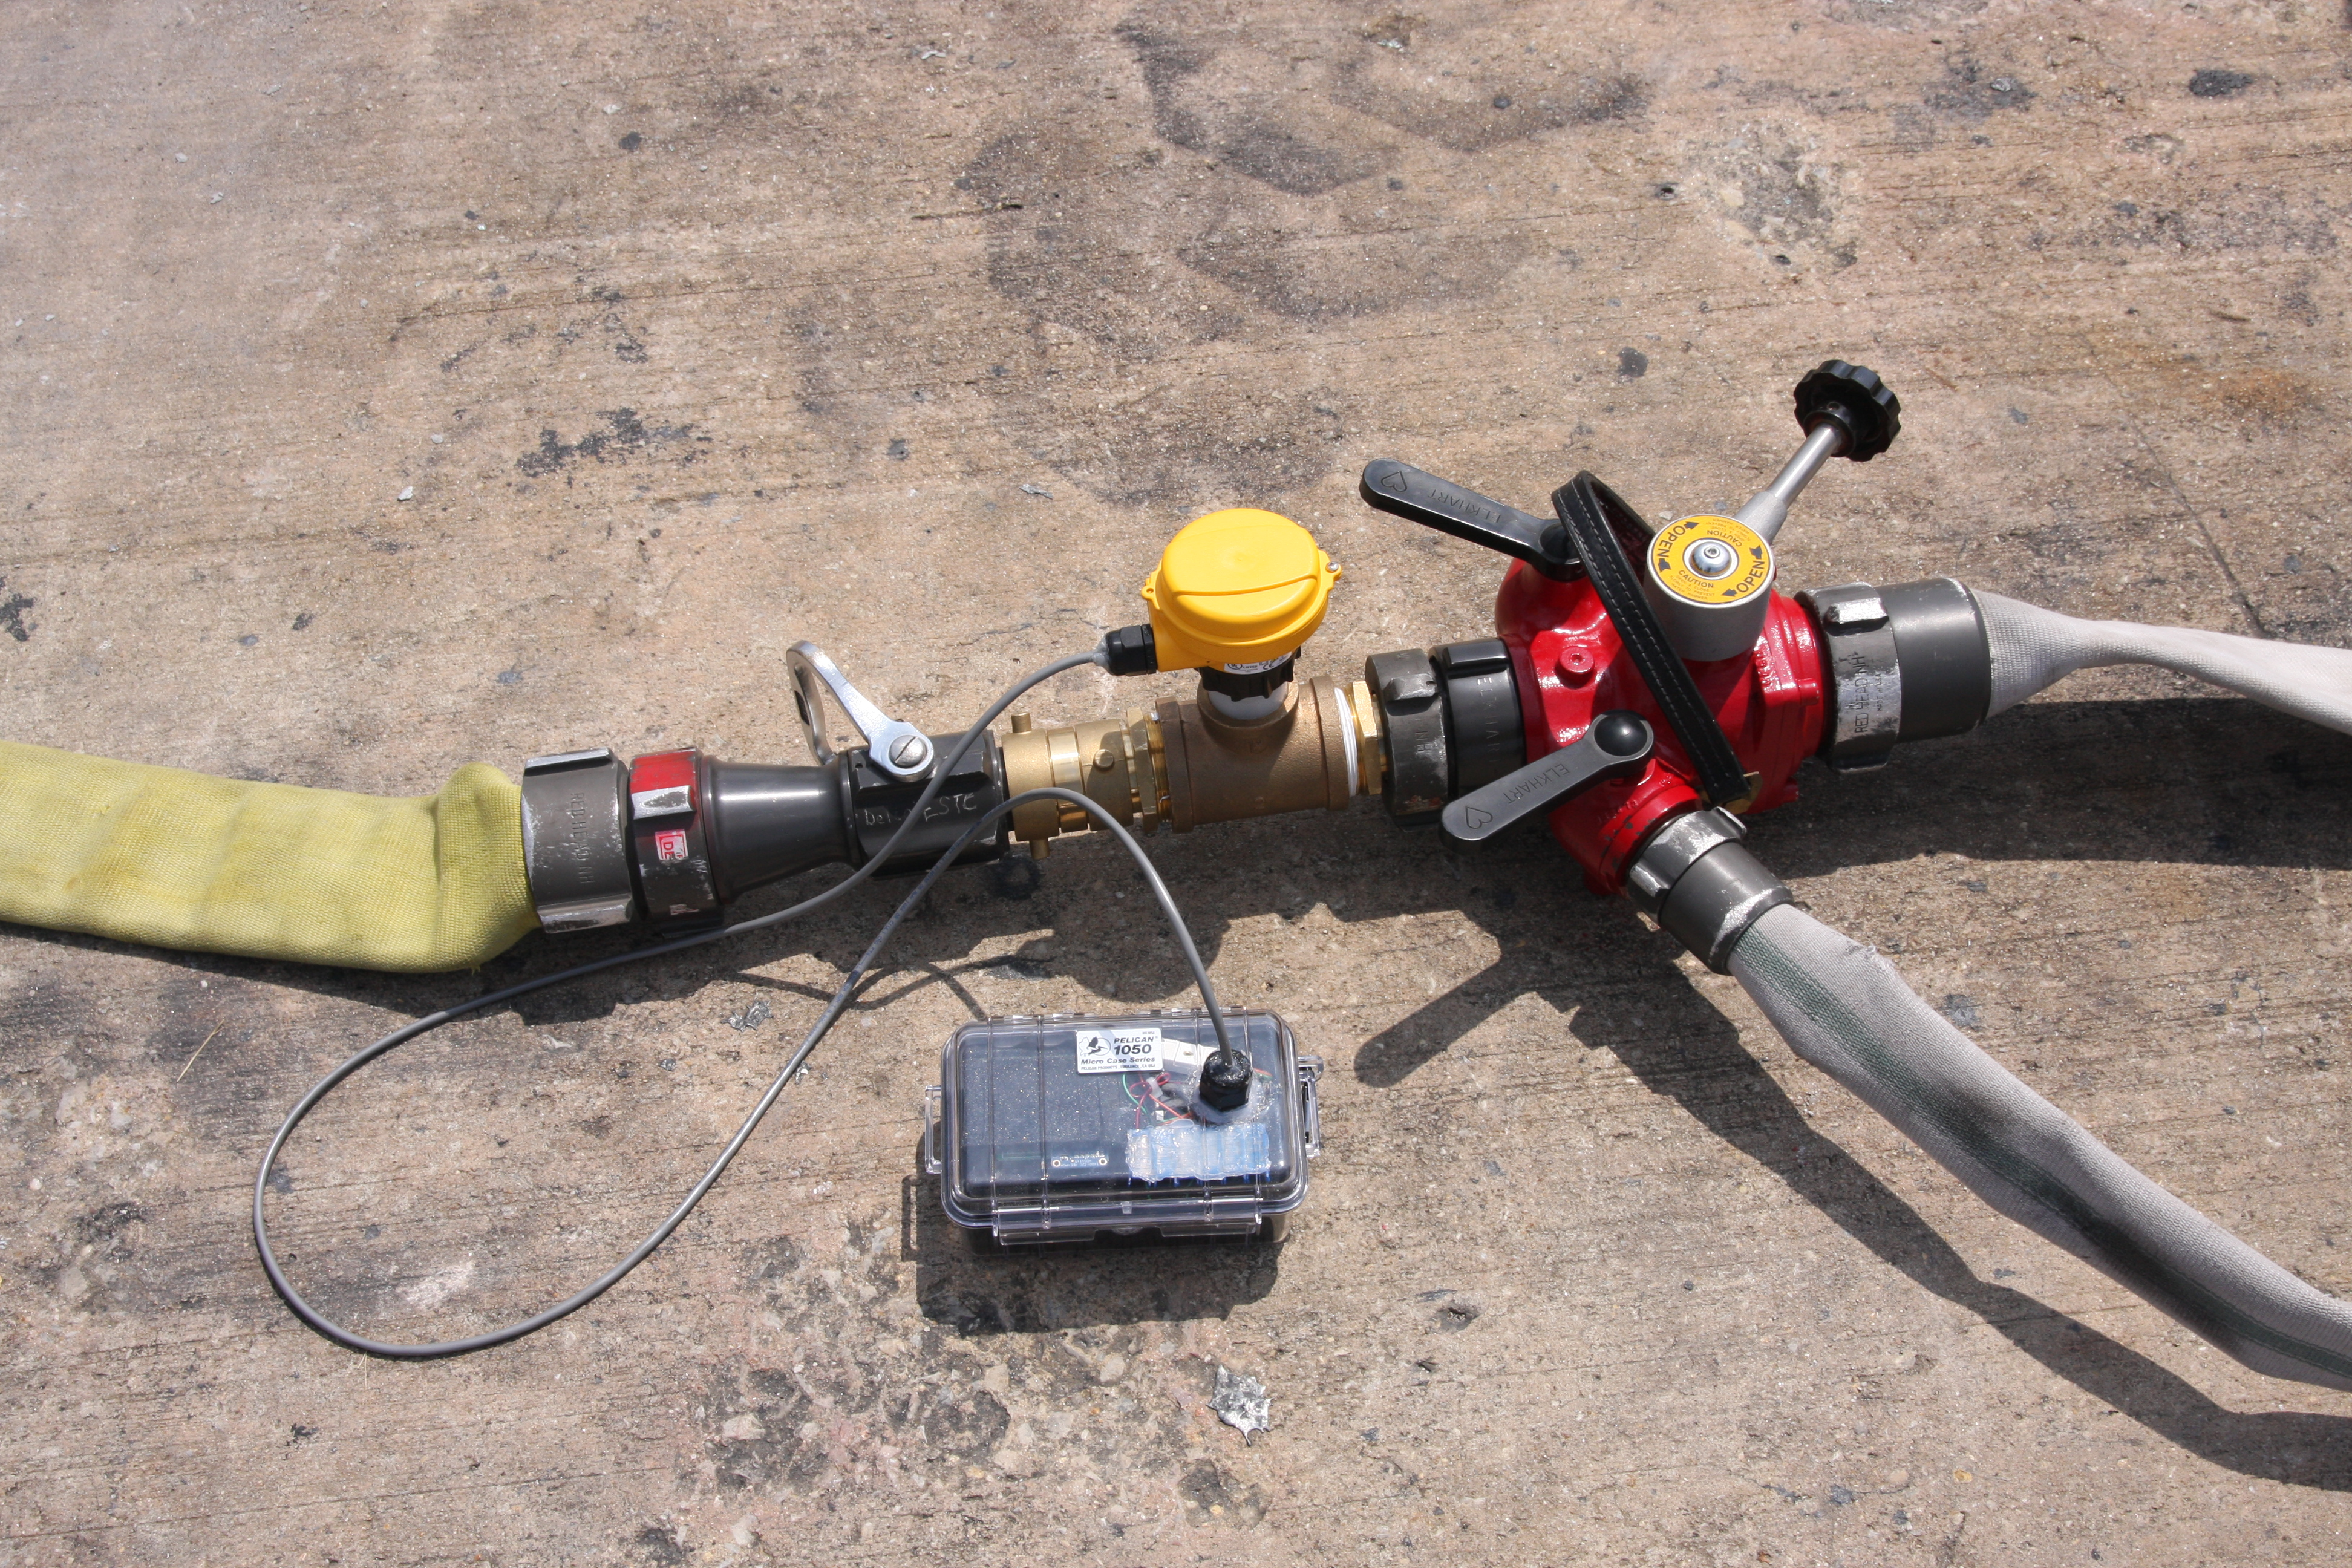
\includegraphics[width=6in]{../../Figures/flow_meter}
%\caption[Picture of Flowrate Meter]{Pressure and flow meter combination used to measure water flowrate}
%\label{fig:flow_meter}
%\end{figure}

In the following sections, the measurements will be presented in graphic and tabular form. In the graphs, an error bar will represent the estimated uncertainty of the measurement. In the tables, the uncertainty will be included in the table of as part of the caption.

\section{Experimental Procedure}
\label{sec:Experimental_Procedure}

\subsection{Cold Flow Experimental Procedure}
\label{sec:Cold_Flow_Procedure}

\subsection{Water Flow Experimental Procedure}
\label{sec:Water_Flow_Procedure}
A variety of experiments were conducted to examine the impact of different hose streams and application methods on air flow inside a structure. All the experiments were conducted in either the East or West Structure; used a monitor or handline with a combination nozzle to flow water in a straight, narrow fog, or wide fog stream pattern; and involved opening and closing doors in the structure to change the ventilation patterns in the structure. Experiments that used a monitor to flow water focused on varying the location of water application, while the experiments that used a handline to flow water focused on varying the pattern in which water was applied.

\subsubsection{East Structure Experiments}
\label{sec:East_Structure_Water_Flow_Procedure}
Five sets of water flow experiments (Tests 29-34) were conducted to observe the impact of different hose streams and application methods on the air flow in the East Structure. Water was flowed from the north side double doors into Room C during Tests 29-32 and from Room C into Room B for Tests 33 and 34. Tests 29 and 30 followed a similar procedure that differed in that Test 29 flowed water from a monitor in a straight stream pattern, while Test 30 flowed water from a monitor nozzle in a narrow fog pattern. 

\subsubsection{West Structure Experiments}
\label{sec:West_Structure_Water_Flow_Procedure}

Four sets of water flow experiments (Tests 16-19) were conducted to observe the impact of using different hose streams and application patterns on the ventilation in the West Structure. Water was flowed from the double doors on the first floor for all experiments. The experiments varied based on flow path configurations and the type of nozzle used. Two flow path configurations were used. Both configurations contained the double doors on the first level in the opened position and the stairwell door and west side double door on the second level being opened and closed depending on the time in the experiment. The main difference between the two configurations was that the first level, south side door was in the opened position for Flow Path Configuration 1 and was in the closed position for Flow Path Configuration 2. Fig.~\ref{fig:flow_path_1} and Fig.~\ref{fig:flow_path_2} contain the floor plan schematics for Flow Path Configuration 1 and Flow Path Configuration 2, respectively.

\begin{figure}[!ht]
\includegraphics[trim=0cm 0cm 0.75cm 4.5cm, clip=true, width=6in]{../../Drawings/PDFs/Without_Instrumentation/West_Structure_Hose_Test_18_1st_Floor}
\\
\includegraphics[trim=0cm 0cm 0.75cm 5cm, clip=true, width=6in]{../../Drawings/PDFs/Without_Instrumentation/West_Structure_Hose_Test_18_2nd_Floor}
\caption[Flow path configuration used during West Structure water flow experiments]{West Structure first floor (top) and second floor (bottom) layouts for Test 18. Both double doors and the south side door were open on the first floor for the duration of the test. On the second floor, the stairwell door and north side, west double door were opened and closed during the experiments, while the north side, east double door and south side door were in the closed position throughout the entire test.}
\label{fig:flow_path_1}
\end{figure}

\begin{figure}[!ht]
\includegraphics[trim=0cm 0cm 0.75cm 4.5cm, clip=true, width=6in]{../../Drawings/PDFs/Without_Instrumentation/West_Structure_Hose_Test_19_1st_Floor}
\\
\includegraphics[trim=0cm 0cm 0.75cm 5cm, clip=true, width=6in]{../../Drawings/PDFs/Without_Instrumentation/West_Structure_Hose_Test_19_2nd_Floor}
\caption[West Structure first and second floor layouts for Test 19]{West Structure first floor (top) and second floor (bottom) layouts for Test 19. Both double doors were open and the south side door was closed on the first floor for the duration of the test. On the second floor, the stairwell door and north side, west double door were opened and closed during the experiments, while the north side, east double door and south side door were in the closed position throughout the entire test.}
\label{fig:flow_path_2}
\end{figure}

\clearpage

The four sets of water flow experiments conducted in the West Structure contained two different procedures for each flow path configuration. One of the procedures involved using a monitor nozzle to flow water at fixed positions in the first floor of the structure, and the other procedure used a handline equipped with a combination nozzle to flow water into the first floor of the structure in various application patterns.  The second procedure used a 1$\frac{3}{4}$" handline equipped with a combination nozzle to flow water in a straight stream, narrow fog stream, and wide fog stream pattern. Each stream was flowed in four different patterns: a fixed position, a sweeping pattern, a clockwise pattern, and a counter clockwise pattern.

\subsubsection{Monitor Nozzle Experimental Procedure}
\label{sec:Monitor_Procedure}
Two sets of the experiments, Tests 16 and 17, involved flowing water from a monitor nozzle in a straight stream, narrow fog stream, and wide fog stream pattern. Each stream was aimed at two different locations on the first floor interior ceiling: the "far target", which was located approximately X m (Xft) from the south interior wall, and the "near target" which was located approximately X m (Xft) from the interior wall of the double doors.

\subsubsection{Handline Experimental Procedure}
\label{sec:Handline_Procedure}
Two sets of experiments, Tests 18 and 19, involved flowing water in different stream patterns from a 1.75" handline equipped with a combination nozzle. Each hose stream was flowed in four different patterns: a fixed position, a sweeping pattern, a clockwise pattern, and a counter clockwise pattern.

Tests 18 and 19 followed identical procedures that involved flowing water from a handline using different hose stream and application pattern combination.  The handline combination nozzle was adjusted to produce three types of hose streams: a straight stream, a narrow fog stream, and a wide fog stream. Tests 18 and 19 involved three sets of experiments, one for each type of hose stream. For each set of experiments, four different application patterns were tested. First, water was applied while the hose was in a fixed position. Next, the hoseline was moved from side-to-side across the open room, creating a sweeping application pattern. Finally, the hoseline was rotated in both the clockwise and counterclockwise directions, creating clockwise and counterclockwise application patterns. 

To begin each set of experiments, the combination nozzle was adjusted to produce the desired hose stream pattern. Once the nozzle was adjusted, water was applied while the hoseline was in the fixed position. After 60 seconds of water flow, the stairwell door was opened. 60 seconds after the stairwell door was opened, the north side, west double door on the second floor was opened, and water continued to flow for 60 more seconds. Then, the hoseline and two doors were closed, and the procedure was repeated for the sweeping, clockwise, and counterclockwise application patterns.

\begin{figure}[!ht]
\includegraphics[width=6in]{../../Figures/Test_18}
\caption[North Side of West Structure during Test 18]{North side of West Structure during Test 18. A straight stream pattern is being applied, and the flow path is fully established with the stairway door and the north side, west double door both opened.}
\label{fig:test_18_pic}
\end{figure}

\clearpage

\chapter{Results}
\label{chap:Results}

\section{Cold Flow Test Results}
\label{sec:Cold_Flow_Test_Results}

\section{Water Flow Test Results}
\label{sec:Water_Flow_Test_Results}


\subsection{Monitor Nozzle Experiments}

Figures \ref{fig:Test_16_BDP_A10_Avg_All}-\ref{fig:Test_17_BDP_A13_Avg_All} contain plots of the average velocity through the stairwell door and \nth{2} level, north side, west double door, measured by the bi-directional probes in each doorway for the two application locations and three hose stream patterns for Tests 16 and 17. 

\begin{figure}[!ht]
\includegraphics[width=6in]{../../Figures/Hose_Test_Figures/Test_16_West_063014_custom_BDP_A10_Avg}
\caption{Average Velocity through Stairwell Door, Test 16, All Streams}
\label{fig:Test_16_BDP_A10_Avg_All}
\end{figure}

\begin{figure}[!ht]
\includegraphics[width=6in]{../../Figures/Hose_Test_Figures/Test_16_West_063014_custom_BDP_A13_Avg}
\caption{Average Velocity through \nth{2} Level, North Side, West Double Door, Test 16, All Streams}
\label{fig:Test_16_BDP_A13_Avg_All}
\end{figure}

\clearpage

\begin{figure}[!ht]
\includegraphics[width=6in]{../../Figures/Hose_Test_Figures/Test_17_West_063014_BDP_A13_Avg}
\caption{Average Velocity through Stairwell Door, Test 17, All Streams}
\label{fig:Test_17_BDP_A10_Avg_All}
\end{figure}

\begin{figure}[!ht]
\includegraphics[width=6in]{../../Figures/Hose_Test_Figures/Test_17_West_063014_BDP_A13_Avg}
\caption{Average Velocity through \nth{2} Level, North Side, West Double Door, Test 17, All Streams}
\label{fig:Test_17_BDP_A13_Avg_All}
\end{figure}

\clearpage

\begin{table}[!ht]
\caption{Average air velocity (m/s) through stairwell door for all hose stream and application location combinations for Tests 16 and 17}
\begin{tabular}{|l|c|c|c|c|}
\cline{2-5}
\multicolumn{1}{c|}{} & \multicolumn{2}{c|}{Test 16} & \multicolumn{2}{c|}{Test 17} \\ \hline
\textbf{Stream} & \textbf{Near} & \textbf{Far} & \textbf{Near} & \textbf{Far} \\ \hline
\textit{Straight} & 
%%%%Test 16%%%% 
0.8 $\pm 0.2$ & 0.9 $\pm 0.2$ & 
%%%%Test 17%%%% 
0.7 $\pm 0.1$ & 0.7 $\pm 0.2$ \\ \hline
\textit{Narrow Fog} & 
%%%%Test 16%%%% 
1.4 $\pm 0.1$ & 1.0 $\pm 0.1$ & 
%%%%Test 17%%%% 
0.8 $\pm 0.2$ & 0.8 $\pm 0.1 $ \\ \hline
\textit{Wide Fog} 	& 
%%%%Test 16%%%% 
1.2 $\pm 0.1$ & 1.4 $\pm 0.1$ & 
%%%%Test 17%%%% 
0.9 $\pm 0.2$ & 0.7 $\pm 0.2$ \\ \hline
\end{tabular}
\label{table:Tests_16_17_BDP_A10_Avgs}
\end{table}

%code for higher resolution in tabulated values
%\textit{Straight} & 0.84 & 0.94 & 0.73 & 0.69 \\ \hline
%\textit{Narrow Fog} & 1.41 & 1.00 & 0.75 & 0.75 \\ \hline
%\textit{Wide Fog} & 1.23 & 1.37 & 0.88 & 0.71 \\ \hline

\begin{table}[!ht]
\caption{Average air velocity (m/s) through \nth{2} level double door for all hose stream and application location combinations for Tests 16 and 17}
\begin{tabular}{|l|c|c|c|c|}
\cline{2-5}
\multicolumn{1}{c|}{} & \multicolumn{2}{c|}{Test 16} & \multicolumn{2}{c|}{Test 17} \\ \hline
\textbf{Stream} & \textbf{Near} & \textbf{Far} & \textbf{Near} & \textbf{Far} \\ \hline
\textit{Straight} 	& 
%%%%Test 16%%%% 
2.8 $\pm 0.6$ & 3.1 $\pm 0.5$ & 
%%%%Test 17%%%% 
2.7 $\pm 0.4$ & 2.3 $\pm 0.8$ \\ \hline
\textit{Narrow Fog} & 
%%%%Test 16%%%% 
4.4 $\pm 0.3$ & 3.3 $\pm 0.4$ & 
%%%%Test 17%%%% 
2.6 $\pm 0.6$ & 2.7 $\pm 0.6$ \\ \hline
\textit{Wide Fog} 	& 
%%%%Test 16%%%% 
3.9 $\pm 0.5$ & 4.4 $\pm 0.3$ & 
%%%%Test 17%%%% 
3.1 $\pm 0.7$ & 2.8 $\pm 0.7$ \\ \hline
\end{tabular}
\label{table:Tests_16_17_BDP_A13_Avgs}
\end{table}

%code for higher resolution in tabulated values
%\textit{Straight} 	& 2.82 & 3.10 & 2.66 & 2.33 \\ \hline
%\textit{Narrow Fog} & 4.39 & 3.26 & 2.58 & 2.68 \\ \hline
%\textit{Wide Fog} 	& 3.92 & 4.37 & 3.14 & 2.76 \\ \hline

\subsection{Handline Experiments}

Figures \ref{fig:Test_18_BDP_A10_Avg_All}-\ref{fig:Test_19_BDP_A13_Avg_All} contain plots of the average velocity through the stairwell door and \nth{2} level, north side, west double door, measured by the bi-directional probes in each doorway for the four application patterns and three hose stream patterns for Tests 18 and 19. 

\begin{figure}[!ht]
\includegraphics[width=6in]{../../Figures/Hose_Test_Figures/Test_18_West_063014_BDP_A10_Avg}
\caption{Average Velocity through Stairwell Door, Test 18, All Streams}
\label{fig:Test_18_BDP_A10_Avg_All}
\end{figure}

\begin{figure}[!ht]
\includegraphics[width=6in]{../../Figures/Hose_Test_Figures/Test_18_West_063014_BDP_A13_Avg}
\caption{Average Velocity through \nth{2} Level, North Side, West Double Door, Test 18, All Streams}
\label{fig:Test_18_BDP_A13_Avg_All}
\end{figure}

\clearpage

\begin{figure}[!ht]
\includegraphics[width=6in]{../../Figures/Hose_Test_Figures/Test_19_West_063014_BDP_A10_Avg}
\caption{Average Velocity through Stairwell Door, Test 19, All Streams}
\label{fig:Test_19_BDP_A10_Avg_All}
\end{figure}

\begin{figure}[!ht]
\includegraphics[width=6in]{../../Figures/Hose_Test_Figures/Test_19_West_063014_BDP_A13_Avg}
\caption{Average Velocity through \nth{2} Level, North Side, West Double Door, Test 19, All Streams}
\label{fig:Test_19_BDP_A13_Avg_All}
\end{figure}

\clearpage

Significant air flow through the stairwell and \nth{2} level double door only occurred when the flow path was complete, or when both doors were in the open position. Tables~\ref{table:Tests_18_19_BDP_A10_Avgs} and \ref{table:Tests_18_19_BDP_A13_Avgs} contain the average air velocity measured by the eight BDPs at the stairwell door and \nth{2} level, double door, respectively, during the time the flow path was complete for each application pattern and hose stream combination used during Tests 18 and 19.

\begin{table}[!ht]
\addtolength{\tabcolsep}{-3.25pt}
\small
\caption{Average air velocity (m/s) through stairwell door for all hose stream and application pattern combinations for Tests 18 and 19}
\begin{tabular}{|l|c|c|c|c|c|c|c|c|}
\cline{2-9}
\multicolumn{1}{c|}{} & \multicolumn{4}{c|}{Test 18} & \multicolumn{4}{c|}{Test 19} \\ \hline
\textbf{Stream} & \textbf{Fixed} & \textbf{Sweeping} & \textbf{Clockwise} & \begin{tabular}{@{}c@{}} \textbf{Counter} \\ \textbf{Clockwise} \\ \end{tabular} & \textbf{Fixed} & \textbf{Sweeping} & \textbf{Clockwise} & \begin{tabular}{@{}c@{}} \textbf{Counter} \\ \textbf{Clockwise} \\ \end{tabular} \\ \hline
%%%%%%%%%%%%%%%%%%%%%%%%%%%%%%%%%%%%%%%%%%%%%%%%%%%%%%%%%%%%%
\textit{Straight} 	& 
%%%%Test 18%%%% 
-0.2 $\pm 0.3$ & 0.5 $\pm 0.2$ & 0.7 $\pm 0.2$ & 0.6 $\pm 0.2$ & 
%%%%Test 19%%%% 
 0.0 $\pm 0.1$ & 0.5 $\pm 0.2$ & 0.7 $\pm 0.2$ & 0.6 $\pm 0.2$ \\ \hline
\textit{Narrow Fog} & 
%%%%Test 18%%%% 
 0.4 $\pm 0.3$ & 1.0 $\pm 0.2$ & 0.8 $\pm 0.2$ & 1.0 $\pm 0.4$ & 
%%%%Test 19%%%% 
 1.2 $\pm 0.3$ & 1.2 $\pm 0.3$ & 1.1 $\pm 0.4$ & 1.2 $\pm 0.2$ \\ \hline
\textit{Wide Fog} 	& 
%%%%Test 18%%%% 
 0.9 $\pm 0.2$ & 0.9 $\pm 0.3$ & 0.9 $\pm 0.3$ & 0.8 $\pm 0.3$ & 
%%%%Test 19%%%% 
 1.0 $\pm 0.2$ & 0.7 $\pm 0.2$ & 0.9 $\pm 0.2$ & 0.9 $\pm 0.2$ \\ \hline
\end{tabular}
\label{table:Tests_18_19_BDP_A10_Avgs}
\end{table}

%code to increase resolution of tabulated values
%\textit{Straight} 	& -0.17 & 0.48 & 0.65 & 0.63 & -0.05 & 0.47 & 0.67 & 0.62 \\ \hline
%\textit{Narrow Fog} & 0.41 & 1.02 & 0.79 & 0.99 & 1.23 & 1.18 & 1.14 & 1.22 \\ \hline
%\textit{Wide Fog} 	& 0.93 & 0.90 & 0.91 & 0.75 & 0.96 & 0.67 & 0.89 & 0.93 \\ \hline

\begin{table}[!ht]
\addtolength{\tabcolsep}{-3.25pt}
\small
\caption{Average air velocity (m/s) through \nth{2} level double door for all hose stream and application pattern combinations for Tests 18 and 19}
\begin{tabular}{|l|c|c|c|c|c|c|c|c|}
\cline{2-9}
\multicolumn{1}{c|}{} & \multicolumn{4}{c|}{Test 18} & \multicolumn{4}{c|}{Test 19} \\ \hline
\textbf{Stream} & \textbf{Fixed} & \textbf{Sweeping} & \textbf{Clockwise} & \begin{tabular}{@{}c@{}} \textbf{Counter} \\ \textbf{Clockwise} \\ \end{tabular} & \textbf{Fixed} & \textbf{Sweeping} & \textbf{Clockwise} & \begin{tabular}{@{}c@{}} \textbf{Counter} \\ \textbf{Clockwise} \\ \end{tabular} \\ \hline
%%%%%%%%%%%%%%%%%%%%%%%%%%%%%%%%%%%%%%%%%%%%%%%%%%%%%%%%%%%%%
\textit{Straight}  &
%%%%Test 18%%%% 
-0.4 $\pm 1.3$ & 1.8 $\pm 1.1$ & 2.5 $\pm 1.1$ & 2.4 $\pm 0.8$ &
%%%%Test 19%%%%					
 0.2 $\pm 0.7$ & 1.6 $\pm 0.5$ & 2.5 $\pm 0.7$ & 2.1 $\pm 0.7$ \\ \hline
\textit{Narrow Fog} & 
%%%%Test 18%%%%
 1.3 $\pm 1.1$ & 3.6 $\pm 0.9$ & 2.6 $\pm 0.8$ & 3.5 $\pm 1.6$ & 
%%%%Test 19%%%%
 4.3 $\pm 1.0$ & 3.5 $\pm 1.0$ & 3.5 $\pm 1.5$ & 3.7 $\pm 0.9$ \\ \hline
\textit{Wide Fog} 	& 
%%%%Test 18%%%%
3.0 $\pm 0.7$ & 3.2 $\pm 1.0$ & 3.1 $\pm 1.1$ & 2.6 $\pm 1.3$ & 
%%%%Test 19%%%%
3.3 $\pm 0.7$ & 2.6 $\pm 0.6$ & 3.1 $\pm 0.6$ & 3.2 $\pm 0.5$ \\ \hline
\end{tabular}
\label{table:Tests_18_19_BDP_A13_Avgs}
\end{table}

%code to increase resolution of tabulated values
%\textit{Straight} 	& -0.43 & 1.75 & 2.46 & 2.40 & 0.20 & 1.60 & 2.47 & 2.10 \\ \hline
%\textit{Narrow Fog} & 1.34 & 3.61 & 2.55 & 3.48 & 4.26 & 3.48 & 3.49 & 3.66 \\ \hline
%\textit{Wide Fog} 	& 3.02 & 3.22 & 3.06 & 2.57 & 3.31 & 2.60 & 3.13 & 3.19 \\ \hline

Notice, there is a significant difference between the average air velocity caused by the fixed straight stream and the velocity caused by the narrow and wide fog streams; the velocities for the narrow and wide fog were always significantly higher than the velocity of the fixed stream. It was only when the hose began to move around that the air velocity through the doorways for the straight stream approached the air velocities associated with the narrow and wide fogs for the corresponding pattern. However, the straight stream hose pattern always resulted in the lowest average air velocity through each doorway for the three different hose streams at each of the four application patterns. 

Another important result shown in Figures \ref{fig:Test_18_BDP_A10_Avg_All} and \ref{fig:Test_19_BDP_A10_Avg_All} and in Tables \ref{table:Tests_18_19_BDP_A10_Avgs} and \ref{table:Tests_18_19_BDP_A13_Avgs} is that there is statistically no significant difference in the amount of air flow through the doorways between rotating the hoseline in the clockwise and counter clockwise directions for the three hose streams tested. 

%\begin{figure}[!ht]
%\includegraphics[width=6in]{../../Figures/Hose_Test_Figures/Test_18_West_063014_BDP_A10_Avg_CW_vs_CCW}
%\caption{Average Velocity of Stairwell Door, Test 18, All Streams, CW vs. CCW}
%\label{fig:Test_18_BDP_A10_Avg_CW_vs_CCW}
%\end{figure}
%
%\begin{figure}[!ht]
%\includegraphics[width=6in]{../../Figures/Hose_Test_Figures/Test_19_West_063014_BDP_A10_Avg_CW_vs_CCW}
%\caption{Average Velocity of Stairwell Door, Test 19, All Streams, CW vs. CCW}
%\label{fig:Test_19_BDP_A10_Avg_CW_vs_CCW}
%\end{figure}
%
%\clearpage
%
%\begin{figure}[!ht]
%\includegraphics[width=6in]{../../Figures/Hose_Test_Figures/Test_18_West_063014_BDP_A13_Avg_CW_vs_CCW}
%\caption{Average Velocity of \nth{2} Level Double Door, Test 18, All Streams, CW vs. CCW}
%\label{fig:Test_18_BDP_A13_Avg_CW_vs_CCW}
%\end{figure}
%
%\clearpage
%
%\begin{figure}[!ht]
%\includegraphics[width=6in]{../../Figures/Hose_Test_Figures/Test_19_West_063014_BDP_A13_Avg_CW_vs_CCW}
%\caption{Average Velocity of \nth{2} Level Double Door, Test 19, All Streams, CW vs. CCW}
%\label{fig:Test_19_BDP_A13_Avg_CW_vs_CCW}
%\end{figure}
%
%\clearpage

\chapter{Conclusions}
\label{chap:Conclusions}

\chapter{Future Work}
\label{chap:Future_Work}

\chapter{Acknowledgments}
\label{chap:Acknowledgments}

\bibliography{../../../Bibliography/FDS_refs,../../../Bibliography/FDS_general}

\appendix

\chapter{Appendix A}

Placeholder


\end{document}
